\documentclass[border=6pt]{standalone}
\usepackage{tikz}
\usetikzlibrary{arrows.meta,positioning,calc}
\begin{document}
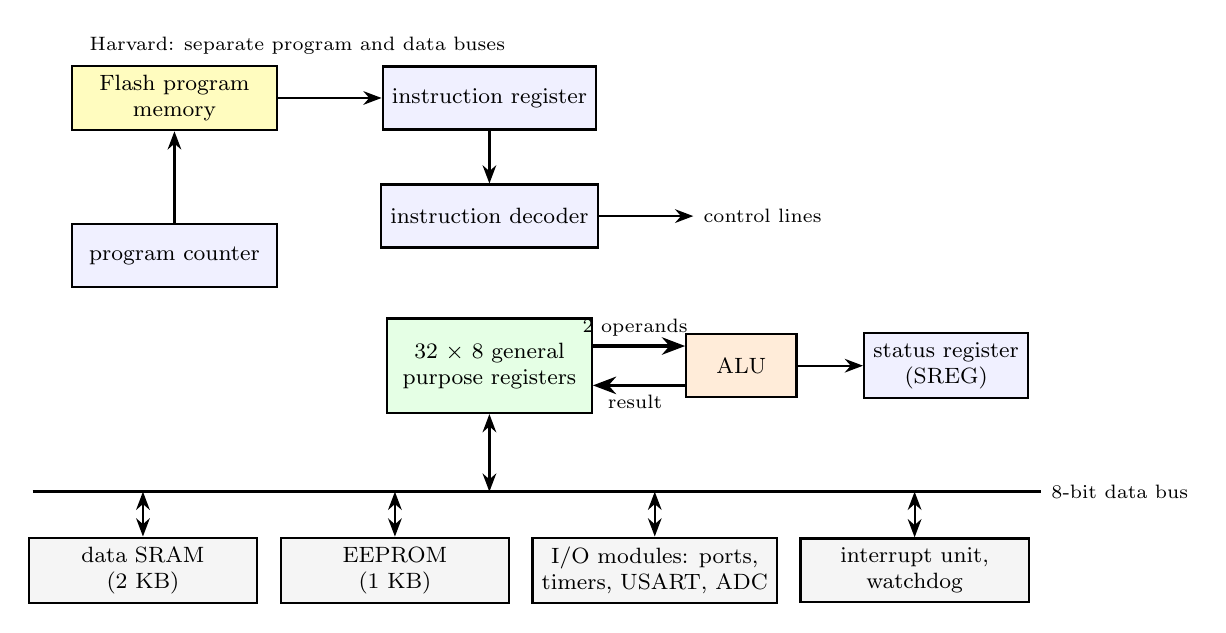
\begin{tikzpicture}[>=Stealth,font=\small,
 b/.style={draw,thick,fill=blue!6,align=center,font=\footnotesize,minimum height=0.8cm,minimum width=2.6cm}]
\node[b,fill=yellow!25] (fl) at (0,0) {Flash program\\memory};
\node[b] (pc) at (0,-2.0) {program counter};
\node[b] (ir) at (4.0,0) {instruction register};
\node[b] (dec) at (4.0,-1.5) {instruction decoder};
\node[b,fill=green!10,minimum height=1.2cm] (rf) at (4.0,-3.4) {32 $\times$ 8 general\\purpose registers};
\node[b,fill=orange!15,minimum width=1.4cm] (alu) at (7.2,-3.4) {ALU};
\node[b,minimum width=2.0cm] (sreg) at (9.8,-3.4) {status register\\(SREG)};
\draw[->,thick] (fl) -- (ir);
\draw[->,thick] (pc) -- (fl);
\draw[->,thick] (ir) -- (dec);
\draw[->,thick] (dec.east) -- ++(1.2,0) node[right,font=\scriptsize]{control lines};
\draw[->,very thick] ($(rf.east)+(0,0.25)$) -- ($(alu.west)+(0,0.25)$);
\draw[<-,very thick] ($(rf.east)+(0,-0.25)$) -- ($(alu.west)+(0,-0.25)$);
\node[font=\scriptsize,anchor=south] at (5.85,-3.15) {2 operands};
\node[font=\scriptsize,anchor=north] at (5.85,-3.65) {result};
\draw[->,thick] (alu) -- (sreg);
% data bus
\draw[very thick] (-1.8,-5.0) -- (11.0,-5.0) node[right,font=\scriptsize]{8-bit data bus};
\draw[<->,thick] (rf.south) -- (4.0,-5.0);
\foreach \x/\t in {-0.4/{data SRAM\\(2 KB)},2.8/{EEPROM\\(1 KB)},6.1/{I/O modules: ports,\\timers, USART, ADC},9.4/{interrupt unit,\\watchdog}} {
  \node[b,fill=gray!8,minimum width=2.9cm] (m) at (\x,-6.0) {\t};
  \draw[<->,thick] (m.north) -- (\x,-5.0);
}
\node[font=\scriptsize,anchor=north west,align=left] at (-1.2,0.9) {Harvard: separate program and data buses};
\end{tikzpicture}
\end{document}
